% Options for packages loaded elsewhere
\PassOptionsToPackage{unicode}{hyperref}
\PassOptionsToPackage{hyphens}{url}
%
\documentclass[
  english,
  man]{apa6}
\usepackage{amsmath,amssymb}
\usepackage{lmodern}
\usepackage{ifxetex,ifluatex}
\ifnum 0\ifxetex 1\fi\ifluatex 1\fi=0 % if pdftex
  \usepackage[T1]{fontenc}
  \usepackage[utf8]{inputenc}
  \usepackage{textcomp} % provide euro and other symbols
\else % if luatex or xetex
  \usepackage{unicode-math}
  \defaultfontfeatures{Scale=MatchLowercase}
  \defaultfontfeatures[\rmfamily]{Ligatures=TeX,Scale=1}
\fi
% Use upquote if available, for straight quotes in verbatim environments
\IfFileExists{upquote.sty}{\usepackage{upquote}}{}
\IfFileExists{microtype.sty}{% use microtype if available
  \usepackage[]{microtype}
  \UseMicrotypeSet[protrusion]{basicmath} % disable protrusion for tt fonts
}{}
\makeatletter
\@ifundefined{KOMAClassName}{% if non-KOMA class
  \IfFileExists{parskip.sty}{%
    \usepackage{parskip}
  }{% else
    \setlength{\parindent}{0pt}
    \setlength{\parskip}{6pt plus 2pt minus 1pt}}
}{% if KOMA class
  \KOMAoptions{parskip=half}}
\makeatother
\usepackage{xcolor}
\IfFileExists{xurl.sty}{\usepackage{xurl}}{} % add URL line breaks if available
\IfFileExists{bookmark.sty}{\usepackage{bookmark}}{\usepackage{hyperref}}
\hypersetup{
  pdftitle={Evidence weighting in confidence judgments for detection and discrimination},
  pdfauthor={Matan Mazor1, Lucie Charles4, Roni Maimon-Mor4,5, \& Stephen M. Fleming1,2,3},
  pdflang={en-EN},
  pdfkeywords={keywords},
  hidelinks,
  pdfcreator={LaTeX via pandoc}}
\urlstyle{same} % disable monospaced font for URLs
\usepackage{graphicx}
\makeatletter
\def\maxwidth{\ifdim\Gin@nat@width>\linewidth\linewidth\else\Gin@nat@width\fi}
\def\maxheight{\ifdim\Gin@nat@height>\textheight\textheight\else\Gin@nat@height\fi}
\makeatother
% Scale images if necessary, so that they will not overflow the page
% margins by default, and it is still possible to overwrite the defaults
% using explicit options in \includegraphics[width, height, ...]{}
\setkeys{Gin}{width=\maxwidth,height=\maxheight,keepaspectratio}
% Set default figure placement to htbp
\makeatletter
\def\fps@figure{htbp}
\makeatother
\setlength{\emergencystretch}{3em} % prevent overfull lines
\providecommand{\tightlist}{%
  \setlength{\itemsep}{0pt}\setlength{\parskip}{0pt}}
\setcounter{secnumdepth}{-\maxdimen} % remove section numbering
% Make \paragraph and \subparagraph free-standing
\ifx\paragraph\undefined\else
  \let\oldparagraph\paragraph
  \renewcommand{\paragraph}[1]{\oldparagraph{#1}\mbox{}}
\fi
\ifx\subparagraph\undefined\else
  \let\oldsubparagraph\subparagraph
  \renewcommand{\subparagraph}[1]{\oldsubparagraph{#1}\mbox{}}
\fi
% Manuscript styling
\usepackage{upgreek}
\captionsetup{font=singlespacing,justification=justified}

% Table formatting
\usepackage{longtable}
\usepackage{lscape}
% \usepackage[counterclockwise]{rotating}   % Landscape page setup for large tables
\usepackage{multirow}		% Table styling
\usepackage{tabularx}		% Control Column width
\usepackage[flushleft]{threeparttable}	% Allows for three part tables with a specified notes section
\usepackage{threeparttablex}            % Lets threeparttable work with longtable

% Create new environments so endfloat can handle them
% \newenvironment{ltable}
%   {\begin{landscape}\centering\begin{threeparttable}}
%   {\end{threeparttable}\end{landscape}}
\newenvironment{lltable}{\begin{landscape}\centering\begin{ThreePartTable}}{\end{ThreePartTable}\end{landscape}}

% Enables adjusting longtable caption width to table width
% Solution found at http://golatex.de/longtable-mit-caption-so-breit-wie-die-tabelle-t15767.html
\makeatletter
\newcommand\LastLTentrywidth{1em}
\newlength\longtablewidth
\setlength{\longtablewidth}{1in}
\newcommand{\getlongtablewidth}{\begingroup \ifcsname LT@\roman{LT@tables}\endcsname \global\longtablewidth=0pt \renewcommand{\LT@entry}[2]{\global\advance\longtablewidth by ##2\relax\gdef\LastLTentrywidth{##2}}\@nameuse{LT@\roman{LT@tables}} \fi \endgroup}

% \setlength{\parindent}{0.5in}
% \setlength{\parskip}{0pt plus 0pt minus 0pt}

% \usepackage{etoolbox}
\makeatletter
\patchcmd{\HyOrg@maketitle}
  {\section{\normalfont\normalsize\abstractname}}
  {\section*{\normalfont\normalsize\abstractname}}
  {}{\typeout{Failed to patch abstract.}}
\patchcmd{\HyOrg@maketitle}
  {\section{\protect\normalfont{\@title}}}
  {\section*{\protect\normalfont{\@title}}}
  {}{\typeout{Failed to patch title.}}
\makeatother
\shorttitle{Evidence weighting in confidence judgments for detection and discrimination}
\keywords{keywords\newline\indent Word count: X}
\DeclareDelayedFloatFlavor{ThreePartTable}{table}
\DeclareDelayedFloatFlavor{lltable}{table}
\DeclareDelayedFloatFlavor*{longtable}{table}
\makeatletter
\renewcommand{\efloat@iwrite}[1]{\immediate\expandafter\protected@write\csname efloat@post#1\endcsname{}}
\makeatother
\usepackage{lineno}

\linenumbers
\usepackage{csquotes}
\ifxetex
  % Load polyglossia as late as possible: uses bidi with RTL langages (e.g. Hebrew, Arabic)
  \usepackage{polyglossia}
  \setmainlanguage[]{english}
\else
  \usepackage[main=english]{babel}
% get rid of language-specific shorthands (see #6817):
\let\LanguageShortHands\languageshorthands
\def\languageshorthands#1{}
\fi
\ifluatex
  \usepackage{selnolig}  % disable illegal ligatures
\fi
\newlength{\cslhangindent}
\setlength{\cslhangindent}{1.5em}
\newlength{\csllabelwidth}
\setlength{\csllabelwidth}{3em}
\newenvironment{CSLReferences}[2] % #1 hanging-ident, #2 entry spacing
 {% don't indent paragraphs
  \setlength{\parindent}{0pt}
  % turn on hanging indent if param 1 is 1
  \ifodd #1 \everypar{\setlength{\hangindent}{\cslhangindent}}\ignorespaces\fi
  % set entry spacing
  \ifnum #2 > 0
  \setlength{\parskip}{#2\baselineskip}
  \fi
 }%
 {}
\usepackage{calc}
\newcommand{\CSLBlock}[1]{#1\hfill\break}
\newcommand{\CSLLeftMargin}[1]{\parbox[t]{\csllabelwidth}{#1}}
\newcommand{\CSLRightInline}[1]{\parbox[t]{\linewidth - \csllabelwidth}{#1}\break}
\newcommand{\CSLIndent}[1]{\hspace{\cslhangindent}#1}

\title{Evidence weighting in confidence judgments for detection and discrimination}
\author{Matan Mazor\textsuperscript{1}, Lucie Charles\textsuperscript{4}, Roni Maimon-Mor\textsuperscript{4,5}, \& Stephen M. Fleming\textsuperscript{1,2,3}}
\date{}


\authornote{

The authors have no conflicting interests to declare.

Correspondence concerning this article should be addressed to Matan Mazor, 12 Queen Square, London WC1N 3BG. E-mail: \href{mailto:mtnmzor@gmail.com}{\nolinkurl{mtnmzor@gmail.com}}

}

\affiliation{\vspace{0.5cm}\textsuperscript{1} Wellcome Centre for Human Neuroimaging, UCL\\\textsuperscript{2} Max Planck UCL Centre for Computational Psychiatry and Ageing Research\\\textsuperscript{3} Department of Experimental Psychology, UCL\\\textsuperscript{4} Institute of Cognitive Neuroscience, UCL\\\textsuperscript{5} FMRIB Centre, Nuffield Department of Clinical Neuroscience, University of Oxford}

\abstract{
Confidence in perceptual decisions is more sensitive to evidence in support of the decision than to evidence against it. This positive evidence bias (PEB) has been demonstrated in confidence ratings in binary discrimination decisions between two stimulus categories. Recent theoretical proposals suggest that a PEB is due to observers adopting a detection-like strategy when rating their confidence, one that has functional benefits for metacognition in real-world settings where detectability and discriminability often go hand in hand. However, it is unknown whether, or how, a PEB is also in play for detection decisions about the presence or absence of a stimulus. In three experiments (one lab-based and two online) we first successfully replicate a PEB in discrimination confidence. We then show that a PEB is observed in detection decisions, where participants report the presence or absence of a stimulus, regardless of its identity. We discuss our findings in relation to models that account for a positive evidence bias as emerging from a confidence-specific heuristic, and alternative models where decision and confidence are generated by the same, Bayes-rational process.
}



\begin{document}
\maketitle

\hypertarget{introduction}{%
\subsection{Introduction}\label{introduction}}

When considering two alternative hypotheses, the probability of a chosen hypothesis to be correct is not only a function of the likelihood of observations under the chosen hypothesis, but also under the unchosen one. For example, when deciding that a random dot motion display was drifting to the right and not to the left, confidence should not only positively weigh motion energy to the right (\emph{positive evidence}), but also negatively weigh motion energy to the left (\emph{negative evidence}). However, when rating subjective confidence, subjects place disproportional weight on evidence in favour of the choice, giving rise to a \emph{positive evidence bias} (Koizumi, Maniscalco, \& Lau, 2015; Peters et al., 2017; Rollwage et al., 2020; Samaha \& Denison, 2020; Sepulveda et al., 2020; Zylberberg, Barttfeld, \& Sigman, 2012). Equivalently, confidence ratings in discrimination are sensitive not only to the \emph{relative evidence} of the chosen hypothesis compared with the unchosen one (also termed \emph{balance of evidence}; see Fig. \ref{fig:RC-2dmodel}, left panel), but also to the \emph{sum evidence} for the two hypotheses (which for perceptual decisions is often related to \emph{visibility}, Rausch, Hellmann, \& Zehetleitner, 2018).



\begin{figure}
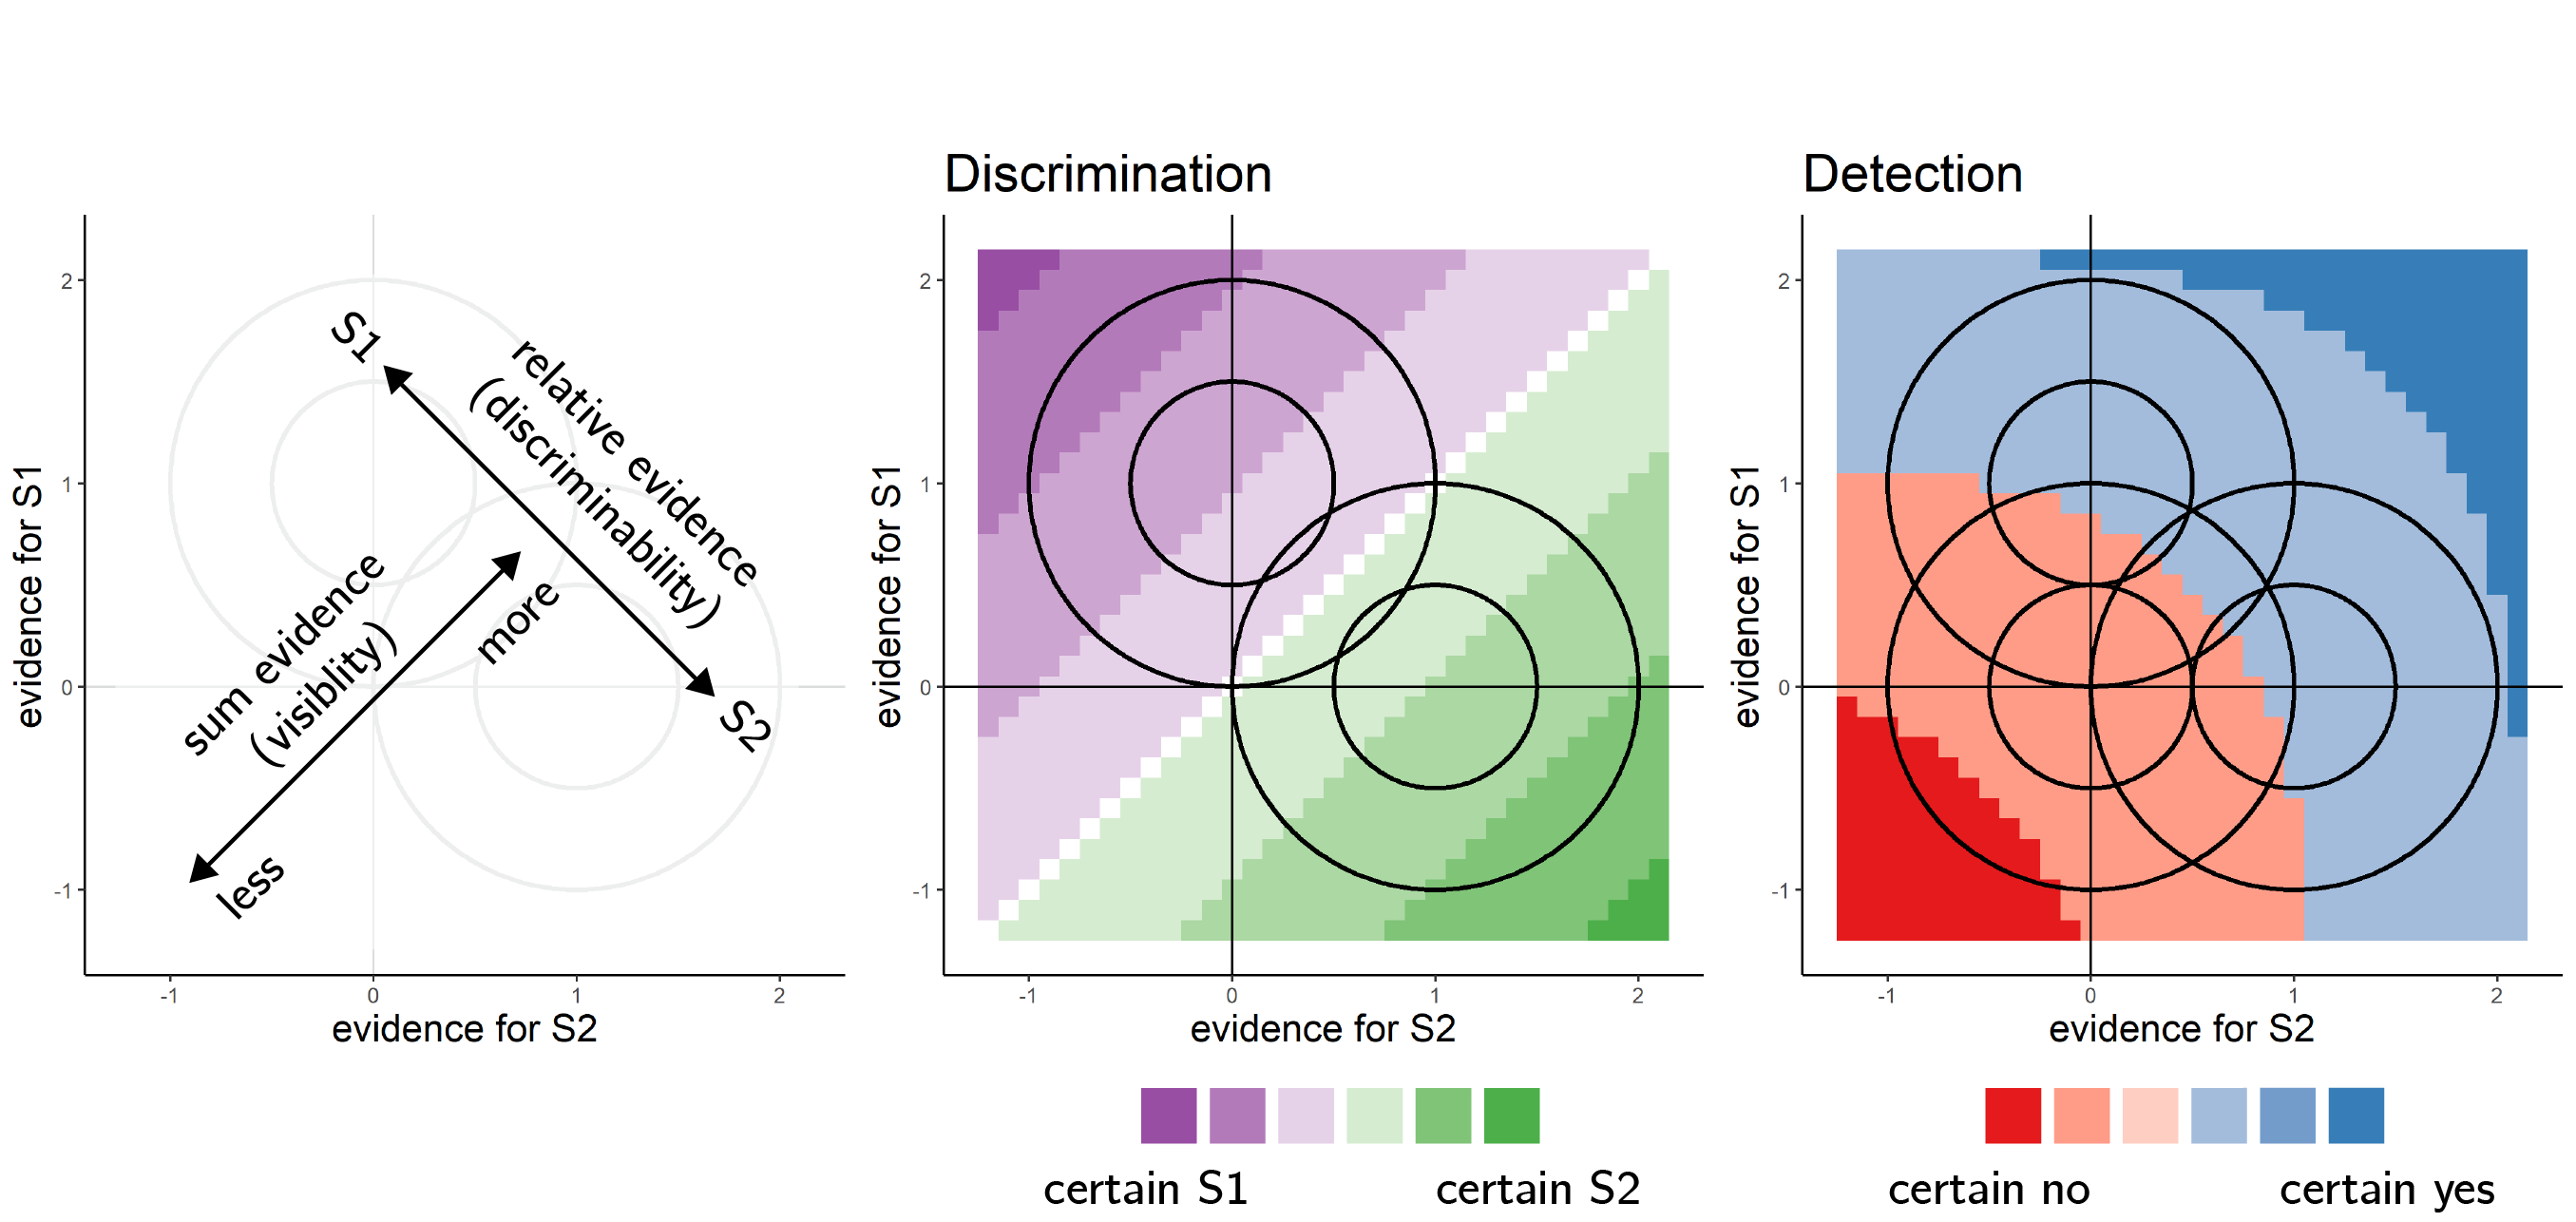
\includegraphics[width=\textwidth]{figures/2dmodel_enhanced} \caption[Discrimination and detection in a two-dimensional SDT model]{Discrimination and detection in a two-dimensional Signal Detection Theory model. Left: in a two-dimensional SDT model, evidence \(e\) is sampled from one of two Gaussian distributions (here centered at (0,1) and (1,0)). We define relative evidence as \(e_{S1}-e_{S2}\) and sum evidence as \(e_{S1}+e_{S2}\). Circles represent contours of two-dimensional distributions. Center and Left: response and confidence accuracy are maximized when based on a log-likelihood ratio for the two stimulus categories. Center: in discrimination, this yields optimal decision and confidence criteria that are based on relative evidence (distance from the main diagonal), irrespective of sum evidence. Right: in detection, this yields optimal decision and confidence that are based on a non-linear interaction between relative and sum evidence. The third circle centred at (0,0) represents the two-dimensional distribution of percepts in the absence of stimuli.}\label{fig:RC-2dmodel}
\end{figure}

To account for this apparently irrational discounting of incongruent evidence in confidence formation, Maniscalco, Peters, and Lau (2016) point out that outside of a lab setting, representational spaces are so high-dimensional that keeping track of evidence for every possible stimulus category is not feasible. For example, to be confident that an object is an apple, one would have to negatively weigh evidence for this object being an orange, a banana, a book and a ferret, among infinitely many other unsupported hypotheses. To resolve this engineering challenge, metacognitive systems may have evolved to positively weigh evidence for the chosen hypothesis, while ignoring conflicting evidence. Such a strategy is reasonable, as in Signal Detection space, samples that are farther away from the origin (high visibility) are on average farther away from the discrimination criterion (high discriminability). This strategy is then carried over to the lab, where decisions are made in low-dimensional representational spaces, and where keeping track of evidence for the two alternative stimulus categories is in fact feasible.

A more recent model identified the origin of this response-congruent heuristic not in this curse of dimensionality, but in the variance structure of perceptual evidence (Miyoshi \& Lau, 2020). In a series of simulations, the authors augmented a two-dimensional Signal Detection model with realistic assumptions about the sensory encoding of signal and noise, most importantly that the variance of signal tends to be higher than that of noise. In these settings, a Response Congruent Evidence (RCE) heuristic provided more accurate confidence judgments, meaning ones that are more aligned with objective accuracy, than a Balance of Evidence (BE) heuristic. Again, this model implies that adopting a detection-like strategy when rating one's confidence might have functional benefits for metacognition.

Notably, both models imply a link between confidence in discrimination, and detection judgments about the presence or absence of a stimulus. In a detection setting where multiple possible target stimuli can appear, the likelihood ratio between stimulus presence and absence is more sensitive to evidence for the detected stimulus (positive evidence) compared to evidence for the absence of other, undetected stimuli (negative evidence; see Fig. \ref{fig:RC-2dmodel}, right panel). Accordingly, recent studies have found that discrimination confidence is detection-like (Rausch, Hellmann, \& Zehetleitner, 2018). Perhaps surprisingly, however, there has been limited focus on the complementary question: do detection decisions share features of discrimination confidence, such as a positive evidence bias? In other words, when faced with a detection task where targets are drawn from two stimulus classes, would detection decisions be sensitive to stimulus visibility (like discrimination confidence is), to the stimulus discriminability, or to both? Moreover, little is known about the properties of \emph{detection} (rather than discrimination) confidence: would confidence in the presence of a target stimulus be susceptible to the same positive evidence bias as confidence in stimulus category? Finally, would detection confidence be sensitive to some form of positive evidence bias not only in decisions about target presence, but also in decisions about target absence?

To examine these questions, we conducted three experiments: one lab-based (N=10, 1800 trials per participant) and two online (N=102 and N=100, 112 and 168 trials per participant, respectively). In all experiments participants made discrimination and detection decisions about noisy stimuli, and rated their confidence in these decisions. Using reverse correlation analysis, we measured the influence of random fluctuations in stimulus energy on both responses and confidence ratings, and tested for the existence of processing asymmetries between `present' and `absent' responses in response time, general confidence, and metacognitive sensitivity (Kellij, Fahrenfort, Lau, Peters, \& Odegaard, 2021; Mazor, Friston, \& Fleming, 2020; Mazor, Moran, \& Fleming, 2021; Meuwese, Loon, Lamme, \& Fahrenfort, 2014). In all three experiments, we replicated previous findings of a positive evidence bias in confidence in discrimination decisions (Zylberberg, Barttfeld, \& Sigman, 2012). In contrast, our understanding of decision and confidence formation in detection evolved and changed following each experiment, as evident in our pre-registration documents. When considering the results of all three experiments together, we conclude that, similar to discrimination confidence, detection decisions and confidence ratings are also sensitive to a positive evidence bias (we use the word bias here to mean a deviation from equal weighting of evidence for the two stimulus categories, and not in the sense of a deviation from rationality). We discuss our findings with respect to recent theoretical proposals regarding the origin of a positive evidence bias in discrimination confidence.

\hypertarget{experiment-1}{%
\subsection{Experiment 1}\label{experiment-1}}

\hypertarget{methods}{%
\subsubsection{Methods}\label{methods}}

\hypertarget{participants}{%
\paragraph{Participants}\label{participants}}

The research complied with all relevant ethical regulations, and was approved by the Research Ethics Committee of University College London (study ID number 1260/003). 10 participants were recruited via the UCL's psychology subject pool, and gave their informed consent prior to their participation. Each participant performed four sessions of 600 trials each, in blocks of 100 trials. Sessions took place on different days and consisted of 3 discrimination blocks interleaved with 3 detection blocks.

\hypertarget{experimental-procedure}{%
\paragraph{Experimental procedure}\label{experimental-procedure}}

The experimental procedure for Exp. 1 largely followed the procedure described in Zylberberg, Barttfeld, and Sigman (2012), Exp. 1. Participants observed a random-dot kinematogram for a fixed duration of 700 ms. In discrimination trials, the direction of motion was one of two opposite directions with equal probability, and participants reported the observed direction by pressing one of two arrow keys on a standard keyboard. In detection blocks participants reported whether there was coherent motion by pressing one of two arrow keys on a standard keyboard. In half of the detection trials dots moved coherently to one of two opposite directions, and in the other half they moved randomly.

In both detection and discrimination blocks, participants indicated their confidence following each decision. Confidence was reported on a continuous scale ranging from chance to complete certainty. To avoid systematic response biases affecting confidence reports, the orientation (vertical or horizontal) and polarity (e.g., right or left) of the scale was set to agree with the type 1 response. For example, following an up arrow press, a vertical confidence bar was presented where `guess' is at the center of the screen and `certain' appeared at the upper end of the scale (see Fig. \ref{fig:RC-exp1-design}).

To control for response requirements, for five subjects the dots moved to the right or to the left, and for the other five subjects they moved upward or downward. The first group made discrimination judgments with the right and left keys and detection judgments with the up and down keys, and this mapping was reversed for the second group. The number of coherently moving dots (`motion coherence') was adjusted to maintain performance at around 70\% accuracy for detection and discrimination tasks independently. This was achieved by measuring mean accuracy after every 20 trials, and adjusting coherence by a step of 3\% if accuracy fell below 60\% or went above 80\%.

Stimuli for discrimination blocks were generated using the exact same procedure reported in Zylberberg, Barttfeld, and Sigman (2012)\footnote{We reused the original Matlab code that was used for Exp. 1 in Zylberberg et. al.~(2012), kindly shared by Ariel Zylberberg.}. Trials started with a presentation of a fixation cross for one second, immediately followed by stimulus presentation. The stimulus consisted of 152 white dots (diameter = \(0.14^\circ\)), presented within a \(6.5^\circ\) circular aperture centered on the fixation point for 700 milliseconds (42 frames, frame rate = 60 Hz). Dots were grouped in two sets of 76 dots each. Every other frame, the dots of one set were replaced with a new set of randomly positioned dots. For each coherence value of \(c'\), a proportion of \(c'\) of the dots from the second set moved coherently in one direction by a fixed distance of \(0.33^\circ\), while the remaining dots in the set moved in random directions by a fixed distance of \(0.33^\circ\). On the next update, the sets were switched, to prevent participants from tracing the position of specific dots. Frame-specific coherence values were sampled for each screen update from a normal distribution centred around the coherence value \(c\) with a standard deviation of 0.07, with the constraint that \(c'\) must be a number between 0 and 1.

Stimuli for detection blocks were generated using a similar procedure, with the only difference being that on a random half of the trials coherence was set to 0\%, without random sampling of coherence values for different frames (see Fig. 1).

To probe global metacognitive estimates of task performance, at the end of each experimental block (100 trials) participants estimated the number of correct responses they have made. Analysis of these global metacognitive estimates is provided in Appendix \ref{global}

\begin{figure}
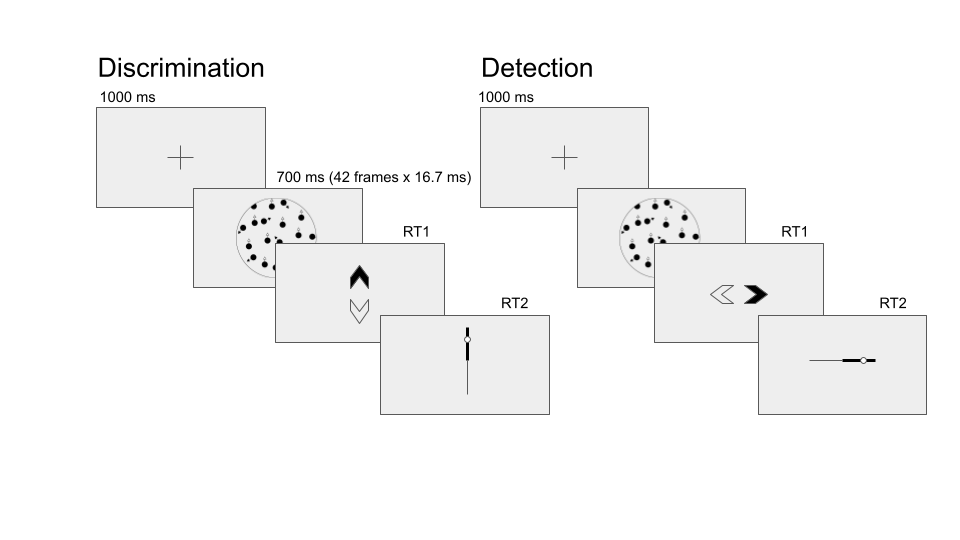
\includegraphics[width=\textwidth]{figures/designExp1} \caption[Experimental design for Exp. 1]{Task design for Experiment 1. In both discrimination and detection blocks, participants viewed 700 milliseconds of a random dot motion array, after which they made a keyboard response to indicate their decision (motion direction in discrimination, signal absence or presence in detection), followed by a continuous confidence report using the mouse. 5 participants viewed vertically moving dots and indicated their detection responses on a horizontal scale, and 5 participants viewed horizontally moving dots and indicated their detection responses on a vertical scale. }\label{fig:RC-exp1-design}
\end{figure}

\hypertarget{randomization}{%
\subsubsection{Randomization}\label{randomization}}

The order and timing of experimental events was determined pseudo-randomly by the Mersenne Twister pseudorandom number generator, initialized in a way that ensures registration time-locking (Mazor, Mazor, \& Mukamel, 2019).

\hypertarget{analysis}{%
\subsubsection{Analysis}\label{analysis}}

Experiment 1 was pre-registered (pre-registration document is available here: \url{https://osf.io/z2s93/}). Our full pre-registered analysis is available in the Appendix.

\hypertarget{reverse-correlation-analysis}{%
\paragraph*{Reverse correlation analysis}\label{reverse-correlation-analysis}}
\addcontentsline{toc}{paragraph}{Reverse correlation analysis}

For the reverse correlation analysis, we followed a procedure similar to the one described in Zylberberg, Barttfeld, and Sigman (2012). For each of the four directions (right, left, up and down), we applied two spatiotemporal filters to the frames of the dot motion stimuli as described in previous studies (Adelson \& Bergen, 1985; Zylberberg, Barttfeld, \& Sigman, 2012). The outputs of the two filters were squared and summed, resulting in a three-dimensional matrix with motion energy in a specific direction as a function of x, y, and time. We then took the mean of this matrix across the x and y dimensions to obtain an estimate of the overall temporal fluctuations in motion energy in the selected direction. Additionally, for every time point we extracted the variance along the x and y dimensions, to obtain a measure of temporal fluctuations in spatial variance. Using this filter, we obtained estimates of temporal fluctuations in the mean and variance of motion energy for upward, downward, leftward and rightward motion within each trial. Given a high correlation between our mean and variance estimates, we focused our analysis on the mean motion energy.

In order to distil random fluctuations in motion energy from mean differences between stimulus categories, we subtracted the mean motion energy from trial-specific motion energy vectors. The mean motion energy vectors were extracted at the group level, separately for each motion coherence level and as a function of motion direction. We chose this approach instead of the linear regression approach used by Zylberberg, Barttfeld, and Sigman (2012) in order to control for nonlinear effects of coherence on motion energy.

\hypertarget{statistical-inference}{%
\paragraph*{Statistical inference}\label{statistical-inference}}
\addcontentsline{toc}{paragraph}{Statistical inference}

Statistics were extracted separately for each participant, and group-level inference was then performed on the first-order statistics. T-test Bayes factors were used to quantify the evidence for the null when appropriate, using a Jeffrey-Zellner-Siow Prior for the null distribution, with a unit prior scale (Rouder, Speckman, Sun, Morey, \& Iverson, 2009).

\hypertarget{results}{%
\subsubsection{Results}\label{results}}

\hypertarget{response-accuracy}{%
\paragraph{Response accuracy}\label{response-accuracy}}

Overall proportion correct was 0.74 in the discrimination and 0.72 in the detection task. Performance for discrimination was significantly higher than for detection (\(M_d = 0.02\), 95\% CI \([0.00\), \(0.04]\), \(t(9) = 2.43\), \(p = .038\)). This difference in task performance reflected a slower convergence of the staircasing procedure for the discrimination task during the first session. When discarding all data from the first session and analyzing only data from the last three sessions (1800 trials per participant), task performance was equated between the two tasks at the group level (\(M_d = 0.00\), 95\% CI \([-0.02\), \(0.02]\), \(t(9) = -0.05\), \(p = .962\); \(\mathrm{BF}_{\textrm{01}} = 3.24\)). In order to avoid confounding differences between discrimination and detection decision and confidence profiles with more general task performance effects, the first session was excluded from all subsequent analyses.

\hypertarget{overall-properties-of-response-time-and-confidence-distributions}{%
\paragraph{Overall properties of response time and confidence distributions}\label{overall-properties-of-response-time-and-confidence-distributions}}

In detection, participants were more likely to respond `yes' than `no' (mean proportion of `yes' responses: \(M = 0.59\), 95\% CI \([0.53\), \(0.64]\), \(t(9) = 3.45\), \(p = .007\)). We did not observe a consistent response bias for the discrimination data (mean proportion of `rightward' or `upward' responses: \(M = 0.52\), 95\% CI \([0.47\), \(0.57]\), \(t(9) = 1.00\), \(p = .344\)).

Replicating previous studies (Kellij, Fahrenfort, Lau, Peters, \& Odegaard, 2021; Mazor, Friston, \& Fleming, 2020; Mazor, Moran, \& Fleming, 2021; Meuwese, Loon, Lamme, \& Fahrenfort, 2014), we find the typical asymmetries between detection `yes' and `no' responses in response time, overall confidence, and the alignment between subjective confidence and objective accuracy (also termed metacognitive sensitivity, here measured as the area under the response-conditional type 2 ROC curve; see Fig. \ref{fig:RC-exp1-asymmetries}). `No' responses were slower compared to `yes' responses (median difference: 85.37 ms), and accompanied by lower levels of subjective confidence (mean difference of 0.08 on a 0-1 scale). Metacognitive sensitivity was higher for detection `yes' compared with detection `no' responses (mean difference in area under the curve units: 0.11). No difference in response time, confidence, or metacognitive sensitivity was found between the two discrimination responses. For a detailed statistical analysis of these behavioural asymmetries see Appendix \ref{appRC:asymmetries1}.



\begin{figure}
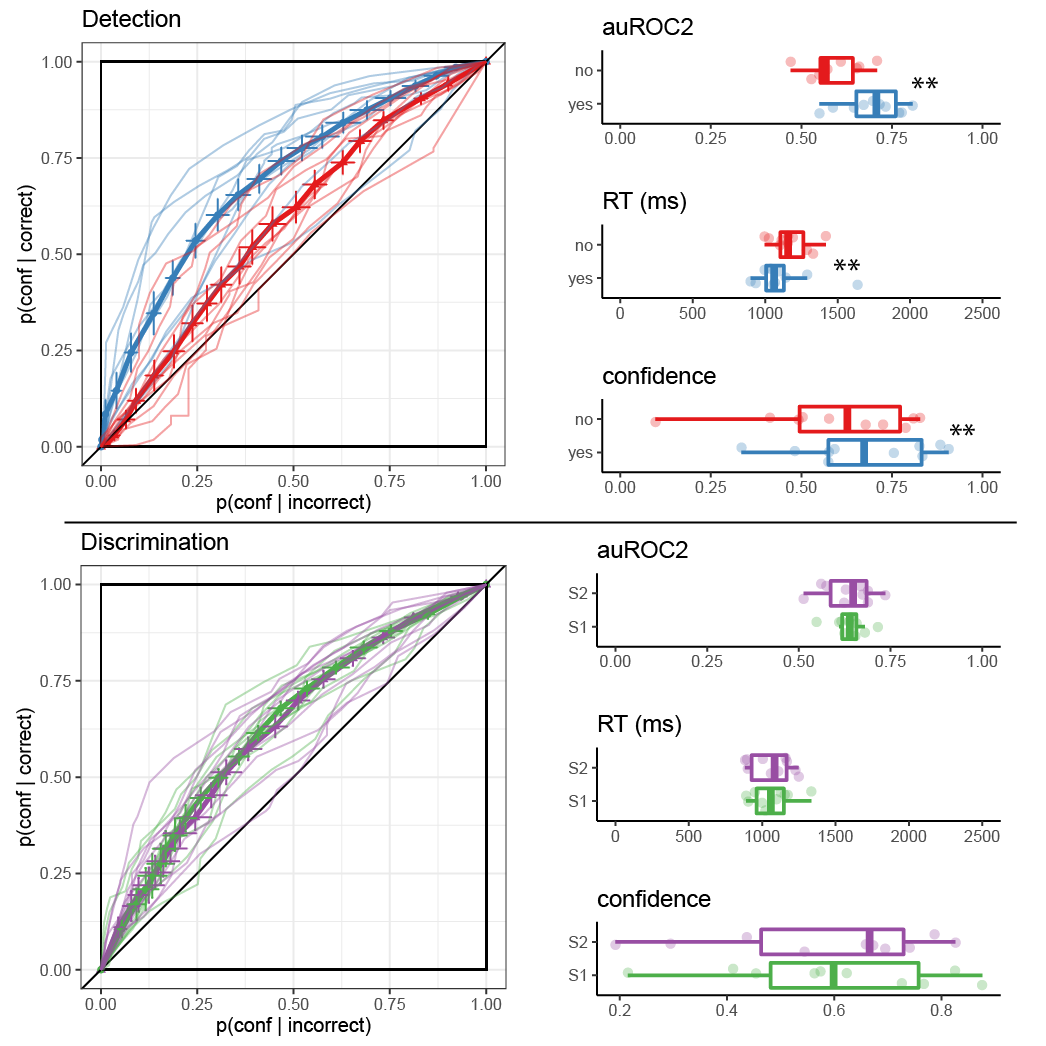
\includegraphics[width=3.49in]{figures/RC-exp1-asymmetries-enhanced} \caption[Behavioural asymmetries in metacognitive sensitivity, response time, and overall confidence, in Exp. 1]{Behavioural asymmetries in metacognitive sensitivity, response time, and overall confidence in detection (upper panel) and discrimination (lower panel), in Exp. 1. Left: Response conditional type 2 ROC curves for the two tasks and four responses in Exp. 1. The area under the type 2 ROC curve is a measure of metacognitive sensitivity, and the difference in areas between the two responses a measure of metacognitive asymmetry. Single-subject curves are presented in low opacity. Right: distributions of the area under the type 2 ROC curve, median response time, and mean confidence for the four responses, across participants. Box edges and central lines represent the 25, 50 and 75 quantiles. Whiskers cover data points within four inter-quartile ranges around the median. Stars represent significance in a two-sided t-test: **: p\textless0.01, ***: p\textless0.001}\label{fig:RC-exp1-asymmetries}
\end{figure}

\hypertarget{reverse-correlation}{%
\paragraph{Reverse Correlation}\label{reverse-correlation}}

Random fluctuations in motion energy made it possible to apply reverse correlation to test which stimulus features are incorporated into decisions and confidence ratings in detection and discrimination. Following Zylberberg, Barttfeld, and Sigman (2012), our statistical analysis focused on the first 300 milliseconds after stimulus onset.



\begin{figure}
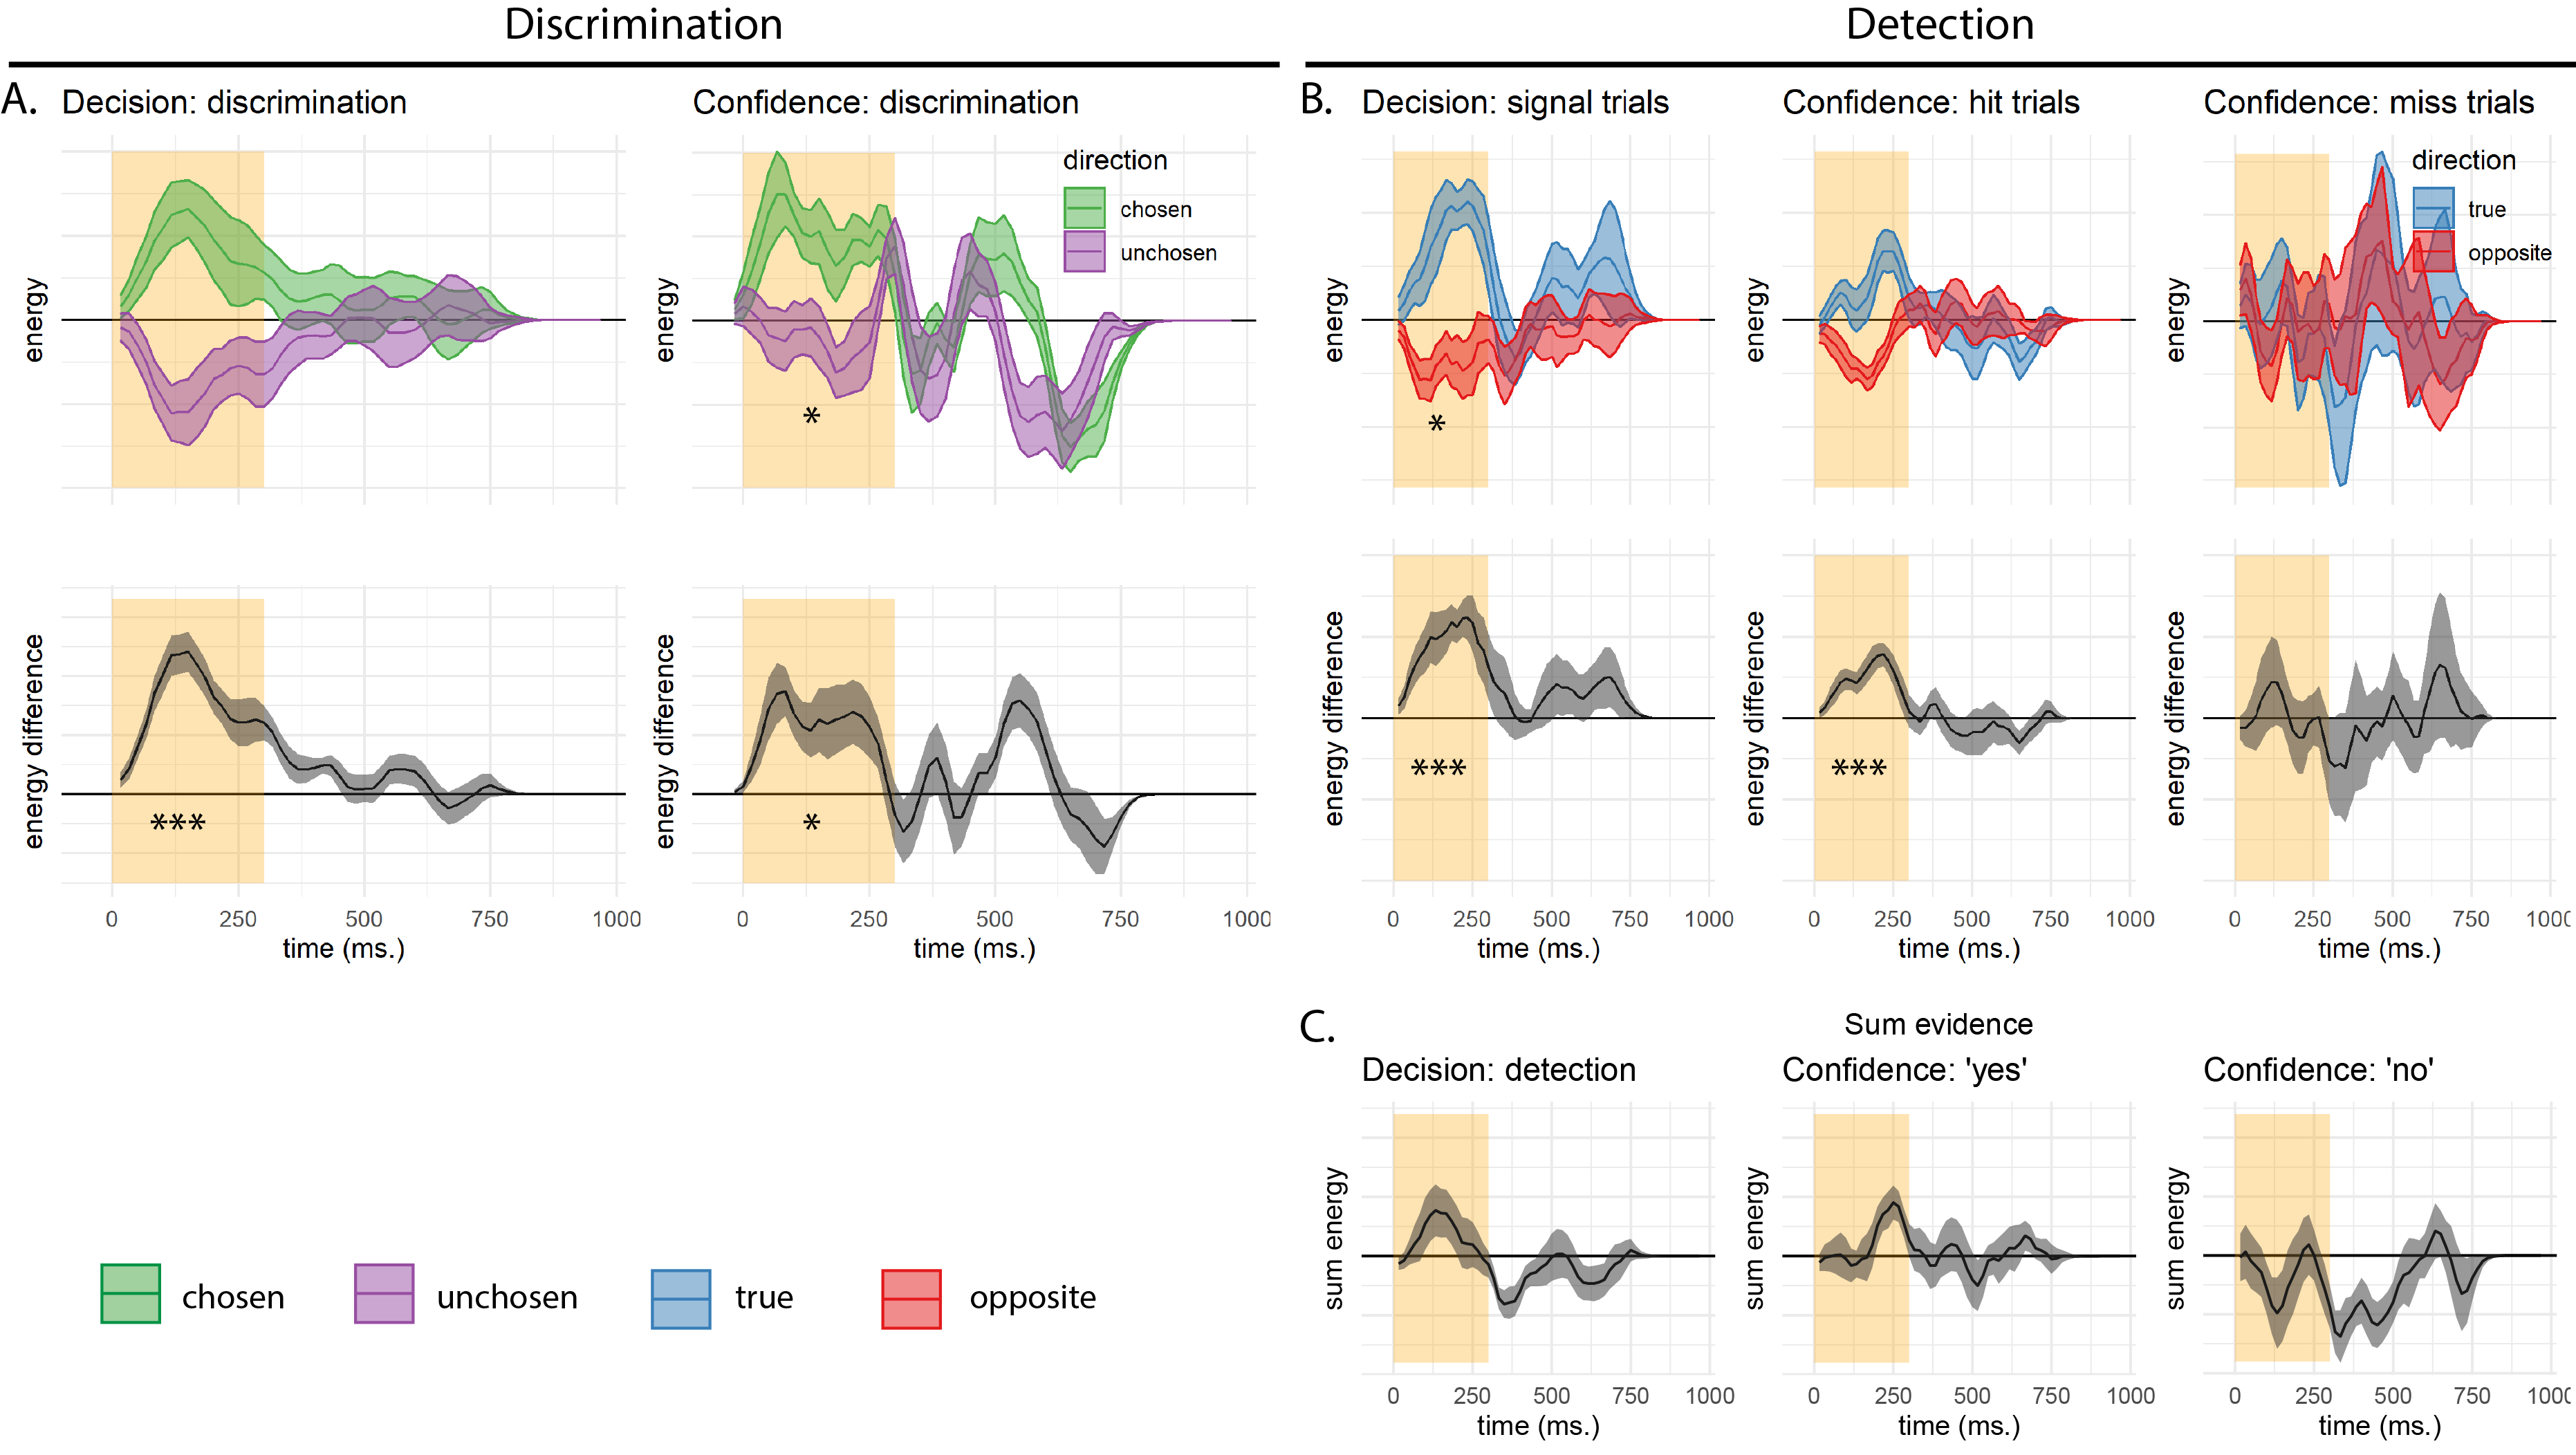
\includegraphics[width=\textwidth]{figures/RC-exp1-RC} \caption[Discrimination and detection in a two-dimensional SDT model]{Reverse correlation, Exp. 1. A: Decision and confidence discrimination kernels. Upper left: motion energy in the chosen (green) and unchosen (purple) direction as a function of time. Lower left: a subtraction between energy in the chosen and unchosen directions. Upper right: confidence effects for motion energy in the chosen (green) and unchosen (purple) directions. Lower right: a subtraction between confidence effects in the chosen and unchosen directions. B: Decision and confidence detection kernels in signal trials. Upper left: difference in motion energy between `yes' and `no' responses in the true (blue) and opposite (red) directions as a function of time. Upper middle and right: confidence effects for motion energy in the true and opposite directions for `yes' and `no' responses, respectively. Lower panels: the subtraction of decision and confidence kernels for the true and opposite directions. C: Decision and confidence detection kernels. Left: difference in sum motion energy between detection `yes' and `no' responses. Middle and right: difference in sum motion energy between high and low confidence trials in `yes' and `no' responses. Shaded areas represent the mean \(\pm\) one standard error. The first 300 milliseconds of the trial are marked in yellow. Stars represent significance in a two-sided t-test: *: p\textless0.05, **: p\textless0.01, ***: p\textless0.001. In the upper rows of panels A and B, stars represent the significance of a positive evidence bias in evidence weighting.}\label{fig:RC-exp1-RC}
\end{figure}

\hypertarget{e1-disc-RC}{%
\subparagraph*{Discrimination}\label{e1-disc-RC}}
\addcontentsline{toc}{subparagraph}{Discrimination}

Using reverse correlation analysis we quantified the effect of random fluctuations in motion energy on the probability of responding `right' and `left' (or `up' and `down'), and on the temporal dynamics of decision formation. Similar to the results obtained by Zylberberg, Barttfeld, and Sigman (2012), participants' decisions were sensitive to motion energy fluctuations during the first 300 milliseconds of the trial (\(t(9) = 7.73\), \(p < .001\); see Fig. \ref{fig:RC-exp1-RC}A, left panels). Note that the green and purple lines are mathematically bound to be symmetric due to the demeaning procedure. To test for a potential asymmetry in evidence weighting in discrimination decisions, we contrasted the contribution of motion energy in the true and opposite directions of motion (defined with respect to the stimulus, and independently of decision). Fluctuations in motion energy in both directions contributed significantly to discrimination decisions (\(t(9) = 8.38\), \(p < .001\)), with no significant difference between them (\(t(9) = -0.65\), \(p = .529\)). In other words, positive and negative evidence equally contributed to discrimination decisions, even when defined independently of the decision.

We then turned to the contribution of motion energy to subjective confidence ratings. The median confidence rating in each experimental session was used to split all motion energy vectors into four groups, according to decision (chosen or unchosen directions) and confidence level (high or low). Confidence kernels for the chosen and unchosen directions were then extracted by subtracting the mean low confidence vectors from the mean high confidence vectors for both the chosen and unchosen directions. We observed a significant effect of motion energy on confidence within the first 300 milliseconds of the trial (\(t(19) = 2.52\), \(p = .021\); see Fig. \ref{fig:RC-exp1-RC}A, right panels). Furthermore, confidence ratings in the discrimination task were more sensitive to motion energy in the chosen direction (positive evidence) than to motion energy in the opposite direction (negative evidence; \(t(9) = 2.81\), \(p = .020\)). This is a replication of the Positive Evidence Bias observed in Zylberberg, Barttfeld, and Sigman (2012).

\hypertarget{detection}{%
\subparagraph*{Detection}\label{detection}}
\addcontentsline{toc}{subparagraph}{Detection}

Carrying out an analogous reverse correlation analysis for detection introduces a challenge: while `no' responses reflect a belief in the absence of any coherent motion, `yes' responses can result from detection of any type of coherent motion going in either direction (or both). We chose to have two possible motion directions in the detection task in order to prevent participants from making `no' responses based on significant motion in an unexpected direction. While this choice ensured that participants cannot trivially accumulate evidence for absence, it also made the reverse correlation analysis more difficult, as we did not have full access to participants' beliefs about the stimulus when they responded `yes.'

As a first approximation, we tested whether sum motion energy along the relevant dimension (horizontal or vertical), regardless of direction (up/down or left/right), affected the probability of a `yes' response. Sum motion energy did not have a significant effect on participants' responses during the first 300 milliseconds (\(t(9) = 1.23\), \(p = .249\); see Fig. \ref{fig:RC-exp1-RC}C, left panel) or at any other time point. The effect of sum motion energy on decision confidence during the first 300 milliseconds was positive and marginally significant (\(t(9) = 2.15\), \(p = .060\); see \ref{fig:RC-exp1-RC}C, middle and right panels). Response-specific effects of sum motion energy on decision confidence were not significant for either response.

\hypertarget{detection-signal-trials}{%
\paragraph*{Detection signal trials}\label{detection-signal-trials}}
\addcontentsline{toc}{paragraph}{Detection signal trials}

A lack of effect of sum motion energy on detection decisions and confidence may be due to the fact that participants were sensitive to relative evidence (e.g., `more dots are moving to the right') rather than to the sum motion along the relevant axis. However, as described above, on any single trial, we cannot tell whether a `yes' response means `I perceived coherent motion to the right' or `I perceived coherent motion to the left.' Instead, in order to approximate participants' belief states during `yes' responses, we focused only on trials in which coherent motion was presented in one of the two directions (signal trials). In these trials, we reasoned that a `yes' response is most likely to reflect the detection of the true direction of motion. We then asked whether fluctuations in the true and opposite directions of motion contributed to detection decision and confidence. This was done by subtracting the motion energy vectors for `yes' and `no' responses in the true and opposite motion directions.

Similar to discrimination decisions, detection decisions were sensitive to perceptual evidence in the first 300 milliseconds of the trial (see Fig. \ref{fig:RC-exp1-RC}B, left panels). However, in contrast to discrimination, an asymmetric evidence weighting was apparent in the decision itself: when deciding whether a stimulus contained coherent motion, participants were more sensitive to fluctuations in motion energy that strengthened the true direction of motion, in comparison to fluctuations that weakened motion in the opposite direction (\(t(9) = 2.31\), \(p = .046\)).

Motion fluctuations in the first 300 milliseconds of the trial also contributed to confidence in detection `yes' responses (contrasting high and low confidence hit trials; \(t(9) = 6.13\), \(p < .001\)). However, unlike in the discrimination task, here we found no positive evidence bias in confidence ratings (\(t(9) = 0.11\), \(p = .913\); see Fig. \ref{fig:RC-exp1-RC}B, middle panels)). To reiterate, while detection decisions were mostly sensitive to fluctuations in motion energy toward the true direction of motion, confidence in detection `yes' responses was equally sensitive to fluctuations in the true and opposite directions of motion.
Confidence in `miss' trials was independent of motion energy (\(t(9) = 0.16\), \(p = .874\)). This was true both for motion energy in the true direction of motion (\(t(9) = 0.12\), \(p = .908\)) as well as for motion energy in the opposite direction (\(t(9) = -0.08\), \(p = .941\)). However, and to anticipate the results of Exp. 3 presented below, we note that this equal weighting of positive and negative evidence in detection confidence was not replicated in a subsequent experiment designed to directly test this surprising result.

\hypertarget{experiment-2}{%
\subsection{Experiment 2}\label{experiment-2}}

In Exp. 1, we replicated previous observations of a positive evidence bias in discrimination confidence, such that evidence in support of a decision was given more weight in the construction of confidence than evidence against it. In contrast, in detection a positive evidence bias was apparent for the decision, but not for the confidence kernels. Equal weighting of positive and negative evidence suggests that detection confidence followed not sum evidence (visibility), but relative evidence (discriminability). Furthermore, confidence in detection `no' responses was not at all affected by fluctuations in motion energy.

In Exp. 2 we tested the robustness of these findings by employing a different type of stimuli (flickering patches) and mode of data collection (a \textasciitilde10 minute online experiment). Our pre-registered objectives (documented here: \url{https://osf.io/8u7dk/}) were 1) to replicate a positive evidence bias in discrimination confidence, 2) to replicate the absence of a positive evidence bias in detection confidence, 3) to replicate the absence of an effect of either positive or negative evidence on confidence in `no' judgments.

\hypertarget{methods-1}{%
\subsubsection{Methods}\label{methods-1}}

\hypertarget{participants-1}{%
\paragraph{Participants}\label{participants-1}}

The research complied with all relevant ethical regulations, and was approved by the Research Ethics Committee of University College London (study ID number 1260/003). 147 participants were recruited via Prolific (prolific.co) and gave their informed consent prior to their participation. They were selected based on their acceptance rate (\textgreater95\%) and for being native English speakers. Following our pre-registration, we aimed to collect data until we had reached 100 included participants based on our pre-specified inclusion criteria (see \url{https://osf.io/8u7dk/}). Our final data set includes observations from 102 included participants. The entire experiment took around 10 minutes to complete. Participants were paid £1.25 for their participation, equivalent to an hourly wage of £7.5.

\hypertarget{experimental-paradigm}{%
\paragraph{Experimental paradigm}\label{experimental-paradigm}}

The experiment was programmed using the jsPsych and P5 JavaScript packages (De Leeuw, 2015; McCarthy, 2015), and was hosted on a JATOS server (Lange, Kuhn, \& Filevich, 2015). It consisted of two tasks (Detection and Discrimination) presented in separate blocks. A total of 56 trials of each task was delivered in 2 blocks of 28 trials each. The order of experimental blocks was interleaved, starting with discrimination.

The first discrimination block started after an instruction section, which included instructions about the stimuli and confidence scale, four practice trials and four confidence practice trials. Further instructions were presented before the second block. Instruction sections were followed by multiple-choice comprehension questions, to monitor participants' understanding of the main task and confidence reporting interface. To encourage concentration, feedback was delivered at the end of the second and fourth blocks about overall performance and mean confidence in the task.

Importantly, unlike the lab-based experiment, there was no calibration of difficulty for the two tasks. The rationale for this is that in Exp. 1 perceptual thresholds for motion discrimination were highly consistent across participants, and staircasing took a long time to converge. Furthermore, in Exp. 1 we aimed to control for task difficulty, but this introduced differences between the stimulus intensity in detection and discrimination. To complement our findings, here we aimed to match stimulus intensity between the two tasks, and accept that task performance might vary.

\hypertarget{trial-structure}{%
\subparagraph*{Trial structure}\label{trial-structure}}
\addcontentsline{toc}{subparagraph}{Trial structure}

In discrimination blocks, trial structure closely followed Exp. 2 from Zylberberg, Barttfeld, and Sigman (2012), with a few adaptations. Following a fixation cross (500 ms), two sets of four adjacent vertical gray bars were presented as a rapid serial visual presentation (RSVP; 12 frames, presented at 25Hz), displayed to the left and right of the fixation cross (see Fig. \ref{fig:RC-exp2-design}). On each frame, the luminance of each bar was randomly sampled from a Gaussian distribution with a standard deviation of 10/255 units in the standard RGB 0-255 coordinate system. For one set of bars, this Gaussian distribution was centered at the same luminance value as the background (128/255). For the other set, it was centered at 133/255, making it brighter on average. Participants then reported which of the two sets was brighter on average using the `D' and `F' keys on the keyboard. After their response, they rated their confidence on a continuous scale, by controlling the size of a colored circle with their mouse. High confidence was mapped to a big, blue circle, and low confidence to a small, red circle. To discourage hasty confidence ratings, the confidence rating scale stayed on the screen for at least 2000 milliseconds. Feedback about response accuracy was delivered after the confidence rating phase.

\begin{figure}
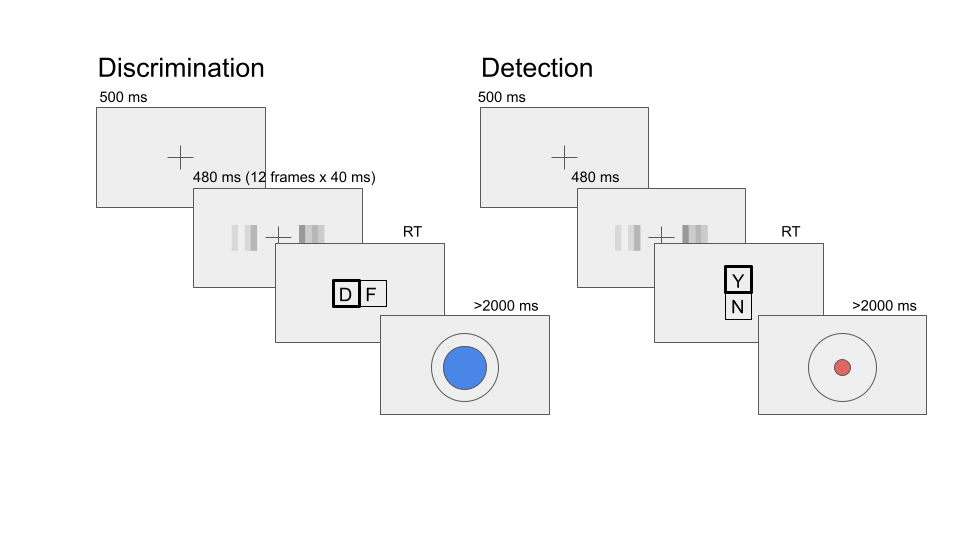
\includegraphics[width=\textwidth]{figures/designExp2} \caption[Experimental design for Exp. 2]{Task design for Experiment 2. In both tasks, participants viewed 480 milliseconds of two flickering patches, after which they made a keyboard response to indicate which of the patches was brighter (discrimination) or whether any of the patches was brighter than the background (detection). }\label{fig:RC-exp2-design}
\end{figure}

Detection blocks were similar to discrimination blocks, with the exception that decisions were made about whether the average luminance of either of the two sets was brighter than the gray background, or not. In `different' trials, the luminance of the four bars in one of the sets was sampled from a Gaussian distribution with mean 133/255, and the luminance of the other set from a Gaussian distribution with mean 128/255. In `same' trials, the luminance of both sets was sampled from a distribution centered at 128/255. Decisions in Detection trials were reported using the `Y' and `N' keys. Confidence ratings and feedback were as in the discrimination task.

\hypertarget{references}{%
\section{References}\label{references}}

\begingroup
\setlength{\parindent}{-0.5in}
\setlength{\leftskip}{0.5in}

\hypertarget{refs}{}
\begin{CSLReferences}{1}{0}
\leavevmode\hypertarget{ref-adelson1985spatiotemporal}{}%
Adelson, E. H., \& Bergen, J. R. (1985). Spatiotemporal energy models for the perception of motion. \emph{Josa a}, \emph{2}(2), 284--299.

\leavevmode\hypertarget{ref-de2015jspsych}{}%
De Leeuw, J. R. (2015). jsPsych: A JavaScript library for creating behavioral experiments in a web browser. \emph{Behavior Research Methods}, \emph{47}(1), 1--12.

\leavevmode\hypertarget{ref-kellij2021investigation}{}%
Kellij, S., Fahrenfort, J., Lau, H., Peters, M. A., \& Odegaard, B. (2021). An investigation of how relative precision of target encoding influences metacognitive performance. \emph{Attention, Perception, \& Psychophysics}, \emph{83}(1), 512--524.

\leavevmode\hypertarget{ref-koizumi2015does}{}%
Koizumi, A., Maniscalco, B., \& Lau, H. (2015). Does perceptual confidence facilitate cognitive control? \emph{Attention, Perception, \& Psychophysics}, \emph{77}(4), 1295--1306.

\leavevmode\hypertarget{ref-lange2015jatos}{}%
Lange, K., Kuhn, S., \& Filevich, E. (2015). Just another tool for online studies (JATOS): An easy solution for setup and management of web servers supporting online studies. \emph{PloS One}, \emph{10}(6), e0130834.

\leavevmode\hypertarget{ref-maniscalco2016heuristic}{}%
Maniscalco, B., Peters, M. A., \& Lau, H. (2016). Heuristic use of perceptual evidence leads to dissociation between performance and metacognitive sensitivity. \emph{Attention, Perception, \& Psychophysics}, \emph{78}(3), 923--937.

\leavevmode\hypertarget{ref-mazor2020distinct}{}%
Mazor, M., Friston, K. J., \& Fleming, S. M. (2020). Distinct neural contributions to metacognition for detecting, but not discriminating visual stimuli. \emph{ELife}, \emph{9}, e53900.

\leavevmode\hypertarget{ref-mazor2019novel}{}%
Mazor, M., Mazor, N., \& Mukamel, R. (2019). A novel tool for time-locking study plans to results. \emph{European Journal of Neuroscience}, \emph{49}(9), 1149--1156.

\leavevmode\hypertarget{ref-mazor2021stage}{}%
Mazor, M., Moran, R., \& Fleming, S. (2021). Stage 2 registered report: Metacognitive asymmetries in visual perception.

\leavevmode\hypertarget{ref-mccarthy2015p5}{}%
McCarthy, L. (2015). p5. js. \emph{URL: Https://P5js. Org}, \emph{3}.

\leavevmode\hypertarget{ref-meuwese2014subjective}{}%
Meuwese, J. D., Loon, A. M. van, Lamme, V. A., \& Fahrenfort, J. J. (2014). The subjective experience of object recognition: Comparing metacognition for object detection and object categorization. \emph{Attention, Perception, \& Psychophysics}, \emph{76}(4), 1057--1068.

\leavevmode\hypertarget{ref-miyoshi2020decision}{}%
Miyoshi, K., \& Lau, H. (2020). A decision-congruent heuristic gives superior metacognitive sensitivity under realistic variance assumptions. \emph{Psychological Review}, \emph{127}(5), 655.

\leavevmode\hypertarget{ref-peters2017perceptual}{}%
Peters, M. A., Thesen, T., Ko, Y. D., Maniscalco, B., Carlson, C., Davidson, M., \ldots{} others. (2017). Perceptual confidence neglects decision-incongruent evidence in the brain. \emph{Nature Human Behaviour}, \emph{1}(7), 1--8.

\leavevmode\hypertarget{ref-rausch2018confidence}{}%
Rausch, M., Hellmann, S., \& Zehetleitner, M. (2018). Confidence in masked orientation judgments is informed by both evidence and visibility. \emph{Attention, Perception, \& Psychophysics}, \emph{80}(1), 134--154.

\leavevmode\hypertarget{ref-rollwage2020confidence}{}%
Rollwage, M., Loosen, A., Hauser, T. U., Moran, R., Dolan, R. J., \& Fleming, S. M. (2020). Confidence drives a neural confirmation bias. \emph{Nature Communications}, \emph{11}(1), 1--11.

\leavevmode\hypertarget{ref-rouder2009bayesian}{}%
Rouder, J. N., Speckman, P. L., Sun, D., Morey, R. D., \& Iverson, G. (2009). Bayesian t tests for accepting and rejecting the null hypothesis. \emph{Psychonomic Bulletin \& Review}, \emph{16}(2), 225--237.

\leavevmode\hypertarget{ref-samaha2020positive}{}%
Samaha, J., \& Denison, R. (2020). The positive evidence bias in perceptual confidence is not post-decisional. \emph{bioRxiv}.

\leavevmode\hypertarget{ref-sepulveda2020visual}{}%
Sepulveda, P., Usher, M., Davies, N., Benson, A. A., Ortoleva, P., \& De Martino, B. (2020). Visual attention modulates the integration of goal-relevant evidence and not value. \emph{Elife}, \emph{9}, e60705.

\leavevmode\hypertarget{ref-zylberberg2012construction}{}%
Zylberberg, A., Barttfeld, P., \& Sigman, M. (2012). The construction of confidence in a perceptual decision. \emph{Frontiers in Integrative Neuroscience}, \emph{6}, 79.

\end{CSLReferences}

\endgroup

Appendix


\end{document}
